\chapter{Conclusion and discussion}
\label{chap:discussion}

\section{Summary of findings}
In language after language, we find three clause types (\diis{}) that are dedicated to three speech acts (assertions, questions, commands). By 18 months old, children seem to be able to differentiate these clause types and associate them with their canonical speech act. To gain this ability, they need to identify the right categories of clauses (i.e.\ solve the clustering problem) and figure out what speech act they are canonically used for (i.e.\ solve the labeling problem). To solve the labeling problem, some speech act information must be available to the learner, but since mismatches are possible -- sentences used to perform speech acts that are not canonically associated with their clause types -- it is not immediately clear how useful it is for learners to be able to identify speech acts, if it is useful at all. To solve the clustering problem, children surely need to pay attention to the surface morpho-syntactic features of each sentence in their input. But in the input that learners actually receive, many surface features might be absent or misleading. Again, it seems plausible that the availability of some information related to speech acts might be helpful to the learner, but this information too is potentially misleading, again due to cases where sentences are used to perform speech acts that are not canonically associated with their clause type.

This dissertation investigates how children figure out clause type categories. In particular, are the surface formal features of the sentences in the input sufficient for children to figure out the clustering of clause types? If not, is speech act information helpful for solving the clustering problem? And how might learners access such speech act information?

I addressed these questions computationally by simulating two learners, a \distlearner{} (\dlearnerabbr{}), and a \praglearner{} (\plearnerabbr{}). Both learners use the surface morpho-syntactic features of the input sentences to attempt to cluster sentences into three categories, i.e.\ to learn the clause type categories. But the \plearnerabbr{} additionally has access to some information about which speech act is performed by a sentence. I found that in English, the \dlearnerabbr{} model could identify interrogative clauses but could not identify the other two clauses, but in Mandarin, this model could not find any of the right categories. The \plearnerabbr{} model in both languages outperforms the \dlearnerabbr{}. In English, the \plearnerabbr{} model can find all three clause types; in Mandarin, the model has problem with imperative clauses. These results suggest that pragmatics is helpful, indeed crucial, to solve the clustering problem. 


%%IMPORTANT, add to chap prosody
Another potential source of information for clause typing is prosody. Indeed, final rises tend to be associated with polar interroagtives cross-linguistically. However, I find that, overall, parents do not use final rises more often with questions. When I incorporate prosodic information into the two models, I find that this information does not improve \dlearnerabbr{'s} performance. Speech act information is still necessary for learners to find the right clause type clustering. When we look at subcategories of interrogatives, polar interroagtievs do have more final rises than declaratives and \twh-interrogatives. A bootstrapping strategy relying on prosody to figure out clause typing would have to be incremental: learners would first come to associate a subset of interrogatives to questions, and then would have to rely on additional correlations in morpho-synatctic and/or pragmatic features to figure out the other interrogatives.

But if the speech act information is useful for clause type learning, how do children figure out speech act information? Given that the way we generally identify a speech act is via its clause type, there is a potentially vicious circle here -- you need to identify a sentence's clause type to infer the speech act that is being performed, but you need to be able to infer speech act information to learn to identify clause types. How do learners avoid this circularity?

One way to break this circularity is to \tit{not} think of the learning of speech acts and clause types as two processes that need to happen sequentially, but as a joint learning process. Children learn to identify speech act and clause type in tandem and mutually informative ways.

To get one step closer to understanding and evaluating this joint learning hypothesis, I first addressed the question of how much speech act information children need to identify clause types. With the \plearnerabbr{} model, I simulated the learning of clause type with various degrees of noise in the speech act information. I showed that even if children can only perceive speech act information a small proportion of the time, they can still benefit from this information, as a noisy pragmatic percept is superior to no pragmatics at all. 



I then explored what kind of non-clause type cues for speech act information are present in the input. Even if children must rely on clause type information to figure out the speech acts, they could have access to additional information that is unrelated to clause typing, but is informative for recognizing speech act type. When speakers perform speech acts, because of the conventional functions of these speech acts on the discourse, the performance might be associated with certain socio-pragmatic features. For example, because of questions' response-elicitation function, we would expect pauses after questions. With prior knowledge about the functions of communication, and expectations about what questions do, children might able to use these socio-pragmatic features to figure out this speech act. If children have such expectations, could they find any useful socio-pragmatic cues in the input? 

I explored two cues that could potentially differentiate questions from other speech acts: pauses and direct eye gaze. I found that parents tend to pause longer after questions, and attend to the child more when asking questions. Therefore it is in principle plausible that there are some socio-pragmatic features that children can use, in addition to their growing knowledge of clause types to infer the speech act category of an utterance. This little bit of information about speech act could then be used to provide the pragmatic boost that the child needs in order to get the clause type clusters identified accurately.


\section{The pragmatic syntactic bootstrapping hypothesis}

As we have discussed, sentential force is an abstract semantic category that is connected to a formal category, clause type, on the one hand, and to speech act on the other. How do they figure out the various sentential forces of their language, i.e., the forms that each force can take (clause types), and the speech acts that they are canonically associated with? 

In Chapter~\ref{chap:introduction}, we have seen that when we put the learning of clause type and learning of speech act together, we seem to run into a chicken-and-egg problem. On the formal side, clause type is an abstract formal feature of a sentence related to a variety of surface forms, none of which is obligatorily present and many of which can occur in sentences with a different clause-type feature. While in principle the surface formal features could be sufficient, this dissertation showed that they in fact fall short. To compensate for this insufficiency, learners can use the speech act information -- which is systematically related to clause types -- to learn to identify clause types and which surface features are relevant for clause typing. 

On the function side, speech act is also an abstract category. As we have seen in Chapter~\ref{chap:eng-sp}, speech act categories are related to a variety of human behaviors (e.g. pauses and eye gaze), none of which are obligatorily present (you don't \emph{need} to pause after a question) and many of which can occur when performing other speech act categories. While I showed that the features are correlated with the use of questions, it is likely that the learners use the clause type information --- which is systematically related to speech acts --- to inform how they infer speech act types.


How can learners break this vicious cycle to figure out the various sentential forces? The hypos{} proposes that the learner can break the cycle by learning clause type and speech act jointly:

%they are both connected to sentential force. 
\begin{exe}\ex\label{ex:prag-syn-hypo}
\tbf{The \hypos{}}:\\
Children jointly learn clause types (and their associated sentential forces) and speech acts from observations of the socio-pragmatic, prosodic, and morpho-syntactic features of input sentences. On the one hand, children learn to identify speech acts by exploiting the prosody of the utterance and the socio-pragmatic features of the utterance (such as the social function of the utterance and the social attentional behavior of the speaker); on the other hand, they learn to identify clause types and their associated sentential force by exploiting the morpho-syntactic features of the sentence. Crucially, however, learning to identify speech acts and learning to identify clause types and sentential forces are mutually informative: children could use speech act information to learn the makeup of clause types and their associated sentential forces, and use clause type information to learn the socio-pragmatics of speech acts.
\end{exe} 

By learning speech act and clause type in tandem and mutually informative ways, we no longer need to assume that learners has to learn one before moving on to the other. Learners can exploit socio-pragmatic features to indirectly identify clause types via identifying the speech act, and exploit the morpho-syntactic features to indirectly identify speech acts via identifying clause types.

In future work, I plan to test the feasibility of this hypothesis computationally by simulating the learning process with a Bayesian clustering model. The proposed model will (i) track the prosodic and socio-pragmatic features of each utterance and infer the speech act that would generate these features; (ii) using knowledge of prosodic and morpho-syntactic features of each sentence, the model will be able to identify the clause type and sentential force that would generate these features; and (iii) speech act on the one hand, and clause type and sentential force on the other, will be inferred jointly. 

Building on this model, we could also probe more into the role of prosody. As discussed in Chapter~\ref{chap:background}, the role of prosody for clause typing might be complicated, which affects how learners might use prosody. There are two possible starting points: learners could either expect prosody (and in particular final rise) to be informative of clause types, especially given the fact that in some languages like Italian, polar interrogatives only differ from declaratives by prosody, or they might not. If not, they might still expect prosody to be indirectly related to clause types by being correlated to speech acts. We can test these options by modifying how prosody is represented in the syntax-pragmatic bootstrapping model mentioned above: in one version, prosodic information depends on both clause type and speech act information, and we can compare this with when the prosodic information only depends on speech act. We can then simulate the learning of languages like Vata, where prosody is not informative of clause typing, and languages like Italian, where prosody is critical for clause typing. 

In this thesis, I've assumed that learners focus on matrix clauses to figure out clause types, and learn to associate them with particular sentential forces. But the same clause types can also occur in embedded contexts, but crucially not with their own sentential force. How do learners eventually relate the two? \textcite{hacquardlidz2018} introduce \hypos{} as a proposal for how children acquire the meaning of attitude verbs. Under their view, learners exploit parallels between syntax and pragmatic function to figure out attitude meanings: namely, the kinds of clause types these verbs embed (in particular whether these embedded clauses share features with matrix declaratives, e.g., \tit{think}), and the kinds of indirect speech acts that these verbs tend to lend themselves to (e.g., indirect assertions for \tit{think}). Thus, learners could first learn to identify clause types by focusing on matrix clauses and associating them with particular speech acts, and later, build on this knowledge to then acquire the meaning of verbs that embed these clauses. 


\section{Conclusion}

This dissertation investigates when and how children figure out the main clause types of their language (declaratives, interrogatives, imperatives) and their sentential forces, and the speech acts they are canonically associated with (assertions, questions, requests). Infants as young as 18 months old seem to be able to differentiate these clause types and associate them with their canonical speech acts. To gain this ability, children need to identify the right categories of clauses (the ``clustering problem") and figure out what functions they are canonically used for (the ``labeling problem"). By comparing a learner with speech act information and one without speech act information, I found that morpho-syntactic and prosodic features are not enough for English learners to find right clause type clustering, and that speech act information is crucial. Similar patterns were found when simulating with Mandarin data. However, the learning of clause types does not require \tit{perfect} speech act information, as noisy speech act information is better than no speech act information. Thus, it is in principle, possible that children learn clause type information while still trying to figure out the speech act information. Additionally, I found that there are socip-pragmatic cues associated with the use of the speech act of questioning. Based on these results, I propose that children learn to figure out clause types and their associated sentential force, and speech acts jointly with observations of morpho-syntactic, prosodic, and socio-pragmatic features: learners use prosodic and morpho-syntactic features, as well as their growing knowledge of speech act information to infer clause types and their related sentential force; meanwhile, they use prosodic and socio-pragmatic features, and their growing knowledge of clause typing to learn about speech acts.  




%%%%%%%%%%%%%
\begin{comment}

If learners expect prosody to be informative of clause types, the case is straightforward for learners of Italian or Portuguese, where polar interrogatives only differ from declaratives by prosody, as they could use the information to find the right clustering. For children learning languages like Vata, where prosody is irrelevant for clause typing in their language, this expectation might be a problem. However, it could be that their input is such that prosodic information is simply uninformative of clause typing. Thus, to test the feasibility of this possibility, we need to look at the input to Vata-acquiring children, and see if assuming the link between prosody and clause type would hinder children from learning the right clause type clustering. 

If children do not assume prosody informs clause typing, Italian- and Portuguese-acquiring children might need to learn the connection between prosody and clause typing, in addition to learning clause type and speech act categories. But it is also possible that children do not need to learn this connection at all. Since children assume prosody informs speech acts, and that speech acts are informative of clause typing, prosodic information could indirectly help the learning of clause type categories. 

Another possibility is that instead of directly informing clause type and/or speech act categories, the learners need to combine prosodic features with some morpho-syntactic features, so that they can find the distinction between polar interrogatives and declaratives. 


In Chapter~\ref{chap:prosody}, I adopted the second strategy, as the speech act information is assumed to be either inaccessible or observable in our current models. As we have seen, prosody does not improve the performance of the \distlearner. But if speech act categories also need to be learned, then we could test how different ways of utilizing prosodic information could influence the learning of clause types and speech acts. Our model also only utilizes one prosodic features, final rise. It's possible that if the model has access to more prosodic features, its performance could improve. 

This leads us to another complication related to prosody, namely languages use different prosodic features for clause typing, and many of them are not correlated with a rising F0 at the end. For example, Akan's breathy termination in fact results in the lowering of F0. Therefore, instead of having a built-in knowledge of the form ``final rise $\sim$ questionhood," children might need to learn to which prosodic features are associated with which speech act/clause type clusters, the same way that they need to learn which morpho-syntactic features go with which clause type cluster.



 
\revise{In this dissertation, I primarily focus on the clause type and speech act of the matrix clauses. This is mostly due to the pragmatical reason that infants at 18 months old might not have figured out embedded clauses yet. The question then is, can we extend our current model to embedded clauses?}

\revise{While the \hypos{} discussed in the previous section is in parallel with the \hypos{} proposed by \textcite{hacquardlidz2018} for the learning of attitude verbs that can embed clauses, it is not straightforward to extend our current discussion with matrix clauses to the embedded clauses. While pragmatics can help learners to figure out matrix clause types, embedded clauses do not have their own speech act information. Additionally, many morpho-syntactic features associated with matrix clauses disappears in embedded contexts. For example, embedded interrogatives no longer have subject-auxiliary inversion:}
\bex{}
Ann knows whether it is raining.
\eex

\revise{However, it is likely that the speech act of the whole utterance still aligns with the clause type of the embedded clause. For example, the speaker is likely asking ``is it raining'' when using \ref{ex:conclusion:embed}. If this is the case, then speech act information might continue helping learners to identify the clause type categories of embedded clauses.}

\bex{ex:conclusion:embed}
I wonder whether it's raining.
\eex

I plan to expand the corpus to include more embedded clauses, and annotate additional features for embedded clauses (e.g. children might have figured out what are complementizers at this point, so we no longer need to lump \tit{whether} with other Unknown Function Items). We can then test what kind of information is needed for children to figure out which surface feature goes with which clause types in embedded contexts.  

 
 
Figure~\ref{fg:model} shows the graphical model. 
  
\begin{figure}[H]
\centering
\begin{tikzpicture}[
  node distance= 0.8cm and 0.8cm,
  classnode/.style={draw,ellipse,text width=0.3cm,align=center},
  enode/.style={draw,ellipse,text width=0.2cm,align=center},
  obsnode/.style={draw,ellipse,text width=0.3cm,align=center, fill=black!30}
]
\node[classnode] (a) {$A$};
\node[obsnode, below right=of a] (p) {$P$};
\node[classnode, below left =of a] (c) {$C$};
\node[obsnode, below left=of c] (s) {$S$};
\node[obsnode, below right =of c] (f) {$F$};
%\node[enode, left=of c] (e) {$e$};
\path (a) edge[-latex] (p)
(a) edge[-latex] (c)
(c) edge[-latex] (s)
(c) edge[-latex] (f)
(a) edge[-latex] (f)
;
\end{tikzpicture}
\caption{Graphical Model}\label{fg:model}
\end{figure}

The question is then whether it is possible for a learner to use the expected social pragmatic cues to initially identify questions in their input, and use this speech act information to bootstrap the process of learning to identify the surface properties of interrogative clauses. The proposed model will (i) track the prosodic and pragmatic features of each utterance and infer the speech act that would generate these features; (ii) using knowledge of prosodic and syntactic features of each sentence, the model will be able to identify the clause type that would generate these features; and (iii) speech and clause type categories will influence each other. The advantage of such a learner is that it can exploit pragmatics to identify clause type indirectly via identifying the speech act, and exploit syntax to identify speech act indirectly via identifying the clause type. 


\revise{}

In our situation, the learners need to figure out two abstract categories, the clause types and the speech acts information, and the =two categories need to be learned in tandem. 

\tbf{The \hypos{}} (alternative):\\
Children learn to identify the sentential force of a sentence by observing the speech acts that the sentence is used to perform on the one hand, and observing the syntactic clause types in tandem and mutually informative ways: children learn to identify clause types by tracking formal regularities in conjunction with their growing knowledge of speech acts and its associated social pragmatic cues; similarly, they identify speech acts by tracking social pragmatic cues in conjunction with their growing understanding of the syntax of clause types. 

because of the systematic mapping between the three major clause types and the three major speech acts, 
The semantic bootstrapping hypothesis states that:
\begin{quote}
[T]he child uses the presence of \tit{semantic} entities such as ``thing,'' ``causal agent,'' ``true in past'' and ``predicate-argument relation'' to infer that the input contains tokens of the corresponding syntactic substantive universals such as \tit{noun}, \tit{subject}, \tit{auxiliary}, \tit{dominates} and so on.\\
\hspace*{\fill} \cite[407]{pinker1987} 
\end{quote}
\end{comment}



\begin{comment}


\bex{}
\ex
\begin{tikzpicture}[level distance=60pt]
\tikzset{every tree node/.style={align=center,anchor=north, font=\scriptsize}}
%}}
\tikzset{level 1/.style={level distance=35pt}}
\tikzset{level 2/.style={sibling distance=35pt}}
%\tikzset{level 3/.style={sibling distance=-6pt}}
%\tikzset{level 4+/.style={sibling distance=-6pt}}
\Tree
[. {Sentential force} 
	[. {Clause type features\\ ([\textpm int, imp])} 
		[. {Surface formal features} ]
		[. {Prosodic features} ]
	]
	[. {Speech act categories \\
	\aqrs{}} 
		
		[. {Prosodic features} ]
		[. {Social pragmatic features} ]
	]
]

\end{tikzpicture}
\eex
\end{comment}



%%%%

%When putting these two together, it first appears that we might have a chicken-and-egg problem: 

